%
% Minimum local register allocation.
%

\documentclass[a4paper, 12pt]{article}
\usepackage[utf8]{inputenc}
\usepackage[serbian]{babel}
\usepackage[hidelinks]{hyperref}
\usepackage{graphicx}
\usepackage{subfig}

\hypersetup{
  colorlinks = true,
  urlcolor = blue,
  linkcolor = blue,
  citecolor = red
}

\begin{document}

\title{Minimalna Lokalna Aloakacija Registra}
\author{Aleksandar Urošević}
\date{\today}
\maketitle

\begin{abstract}
Ovaj rad istražuje problem minimalne lokalne aloakcije registra, fokusirajući se na optimizaciju alokacije registra unutar blokova koda bez skokova. Cilj je pronaći alokaciju koja minimizuje troškove učitavanja i čuvanja podataka, koristeći ograničeni skup dostupnih registara. Ovaj problem je značajan za optimizaciju kompilatora i interpretera. Prethodni radovi na ovu temu pokazuju da je ovaj problem NP težak \cite{OnLocalRegisterAllocation}. Postoje razna rešenja ovog problema, poput pretvaranja problema u rešavanje puzla \cite{RegisterAllocationByPuzzleSolving}. U ovom radu se pradstavlja rešenje zasnovano na genetskom programiranju.
\end{abstract}

\section{Opis problema}
Problem o kojem se diskutuje je problem nalaženja najjeftinijeg načina isvršavanja bloka koda (bez skokova). Pretpostavljamo da imamo na raspolaganju $N$ registara, i $S_i$ ($1 \leq i \leq N$) troškove pri učitavanju ili čuvanja registra $i$. Za datu sekvencu instrukcija programa treba pronaći optimalnu strategiju učitavanja i čuvanja registra tokom izvršavanja programa. 

Sledi opis problema jednim primerom (\ref{primer1}). Ovaj program je identican kao primer iz literature \cite{EvaluationOfAlgorithmsForLocalRegisterAllocation}.

\begin{figure}
\centering
\textbf{Ilustracija}\par\medskip
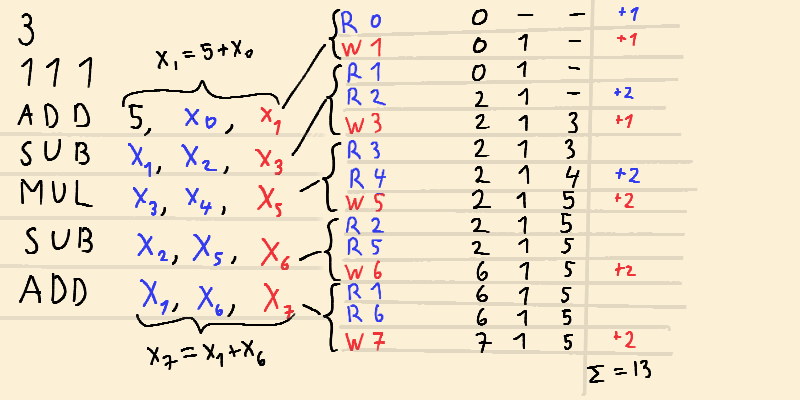
\includegraphics[scale=0.45]{Image/Illustration1}
\caption{Primer 1}
\label{primer1}
\end{figure}

Instrukcija programa $ADD\ x, y, z$ (kao i ostale instrukcije) označava da je neophodno imati promenljive $x, y$ učitanim u registre i neophodno je zapisati novi podatak u $z$. Ova instrukcija moze da bude prevod linije koda $z=x+y$.\\
Cena učitavanja vrednosti u registar je $S_i$. Ukoliko su svi registri puni, neophodno je sačuvati vrednost registra i zameniti je novom potrebnom vrednošću, cena ove procedure je $S_i+S_i=2S_i$, jedno čitanje i jedno pisanje.\\
U desnoj koloni zapisani su koraci koje bi procesor računara izvrsio, predstavljen je optimalno rešenje dobijeno genetskim algoritmom. Ovaj rezultat je potvrdjeno optimalan putem iscrpne pretrage.

Postoje mnogo ranijih radova na ovom problemu. Od interesanthin radova je „Register Allocation by Puzzle Solving“ gde se diskutuje praktično rešavanje generalnog problema alokacija registra (ne samo lokalnog), i to prevođenjem probema na problem rešavanje puzla\cite{RegisterAllocationByPuzzleSolving}. Ovo daje ideju da redove instrukcija mozemo da posmatramo kao blokove koje slažemo. Možemo osmisliti rešenje korišćenjem genetskog programiranja.\\
Funkcija cilja je suma cena korišćenja registara. Možemo je izračunati prolazeći redom kroz niz alokacija registara rešenja, od prvog reda pa do poslednjeg, posmatrajući kada se i kako registri menjaju.\\
Ukrštanje implementiramo biranjem nasumičnog broja $i$ td. $0 \leq i < N$, zamenjujemo sve nizove alokacija $Aj$ sa $Bj$ za sve $i \leq j < N$ (\ref{primer2})\\
Mutacija je implementirana nasumičnim biranjem broja $i$ td. $0 \leq i < N$ koji predstavlja polazni red programa od kojeg nasumično gradimo ostatak niza alokacije.\\


\begin{figure}
\centering
\textbf{Ilustracija}\par\medskip
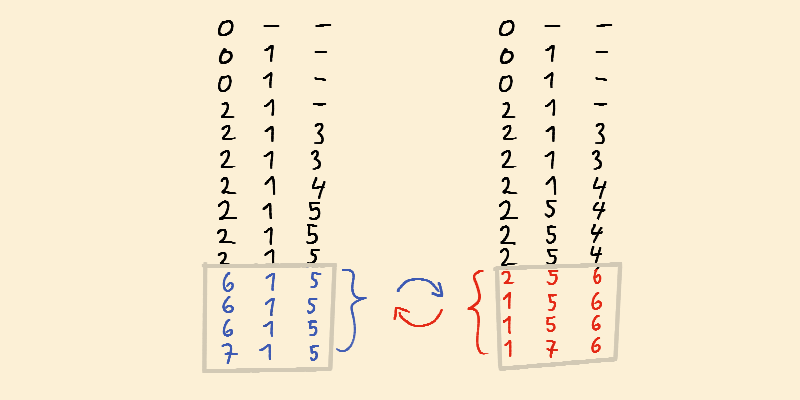
\includegraphics[scale=0.45]{Image/Illustration2}
\caption{Primer 2}
\label{primer2}
\end{figure}


\newpage

\section{Rezultati}

Primenom genetskog programiranja na prvi primer koji je dat i u literaturi \cite{OnLocalRegisterAllocation} dobijamo optimalna rešenja za mali broj iteracija (uz sreću), iscrpa pretraga je takodje prikazana na figuri \ref{methodexample1}.

\begin{figure}
\centering
\subfloat[\centering genetičko programiranje]{{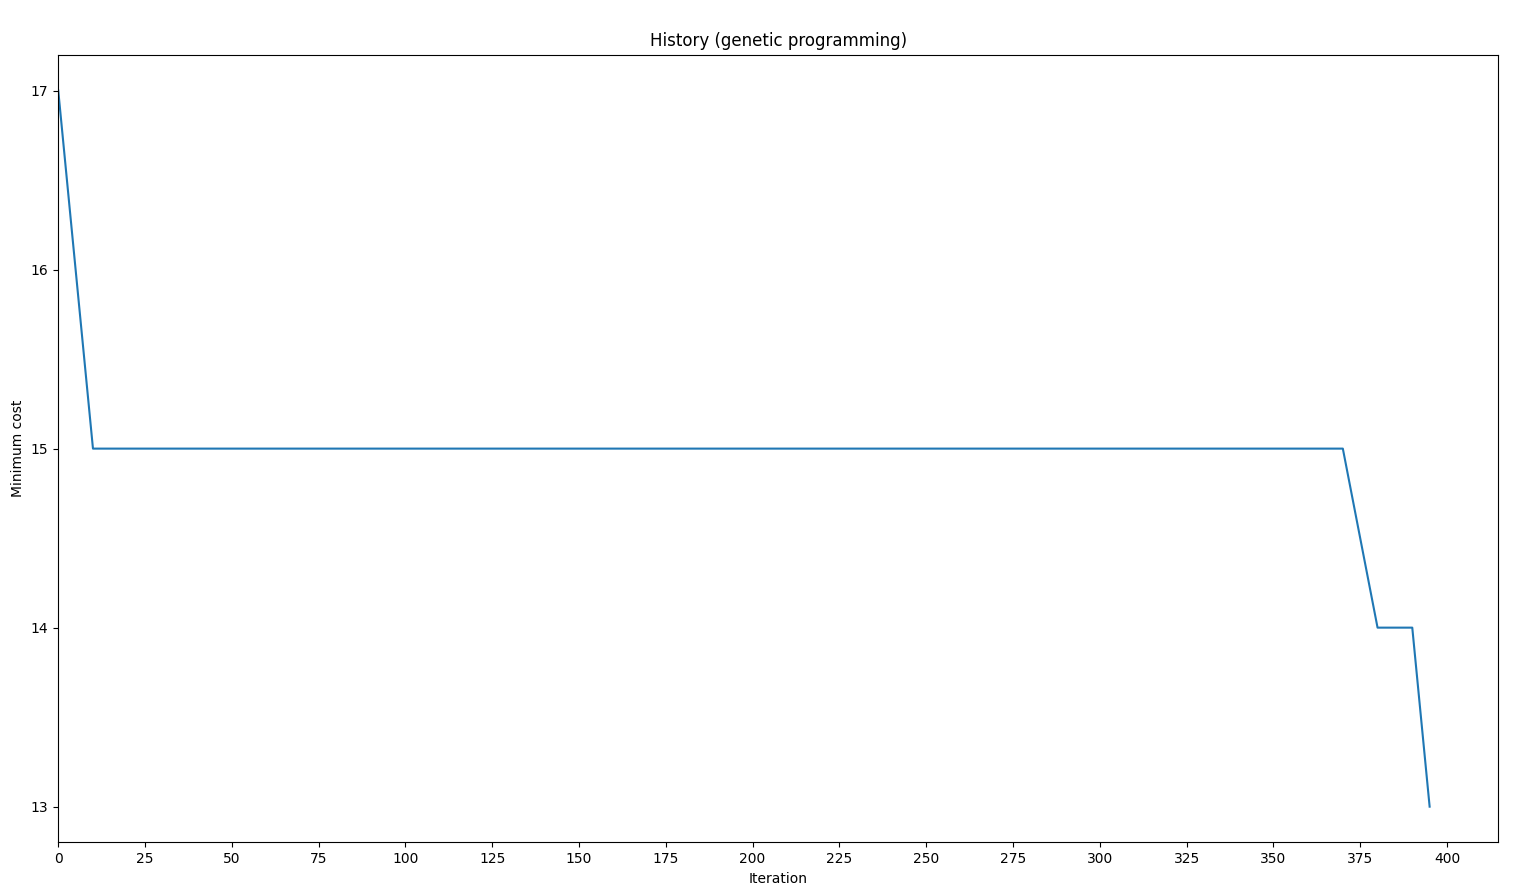
\includegraphics[scale=0.125]{Image/Snapshot/GeneticProgramming1}}}
\qquad
\subfloat[\centering iscrpna pretraga]{{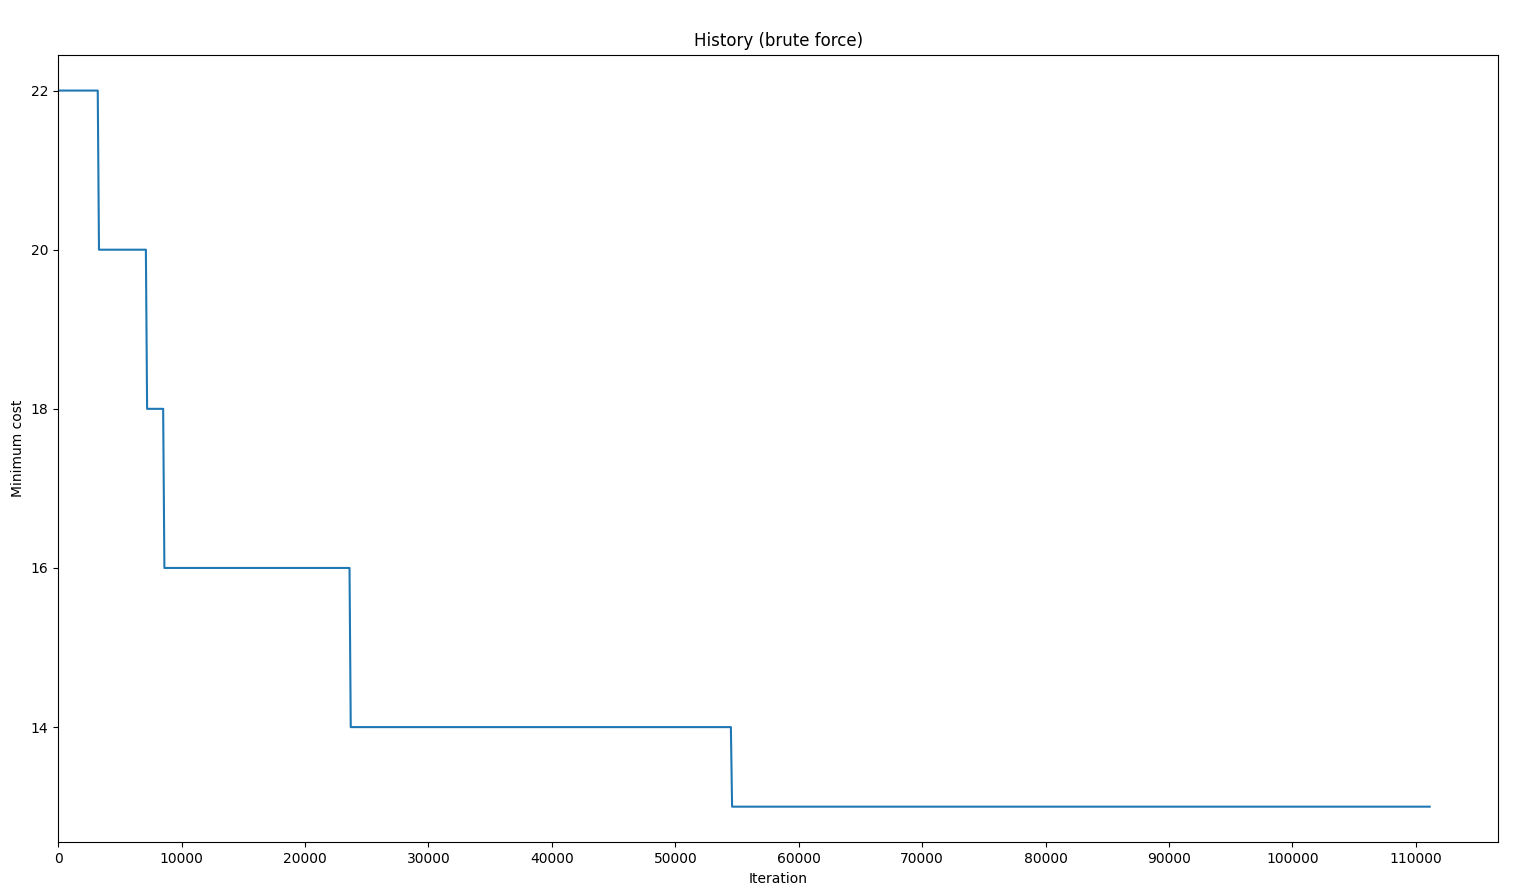
\includegraphics[scale=0.125]{Image/Snapshot/Bruteforce1}}}
\caption{Primena genetičkog programiranja i iscrpne pretrage na primer 1}
\label{methodexample1}
\end{figure}

Na figuri \ref{methodexample2} prikazani su rezultati za veći primer koji se ne nalazi u literaturi.

\begin{figure}
\centering
\subfloat[\centering genetičko programiranje]{{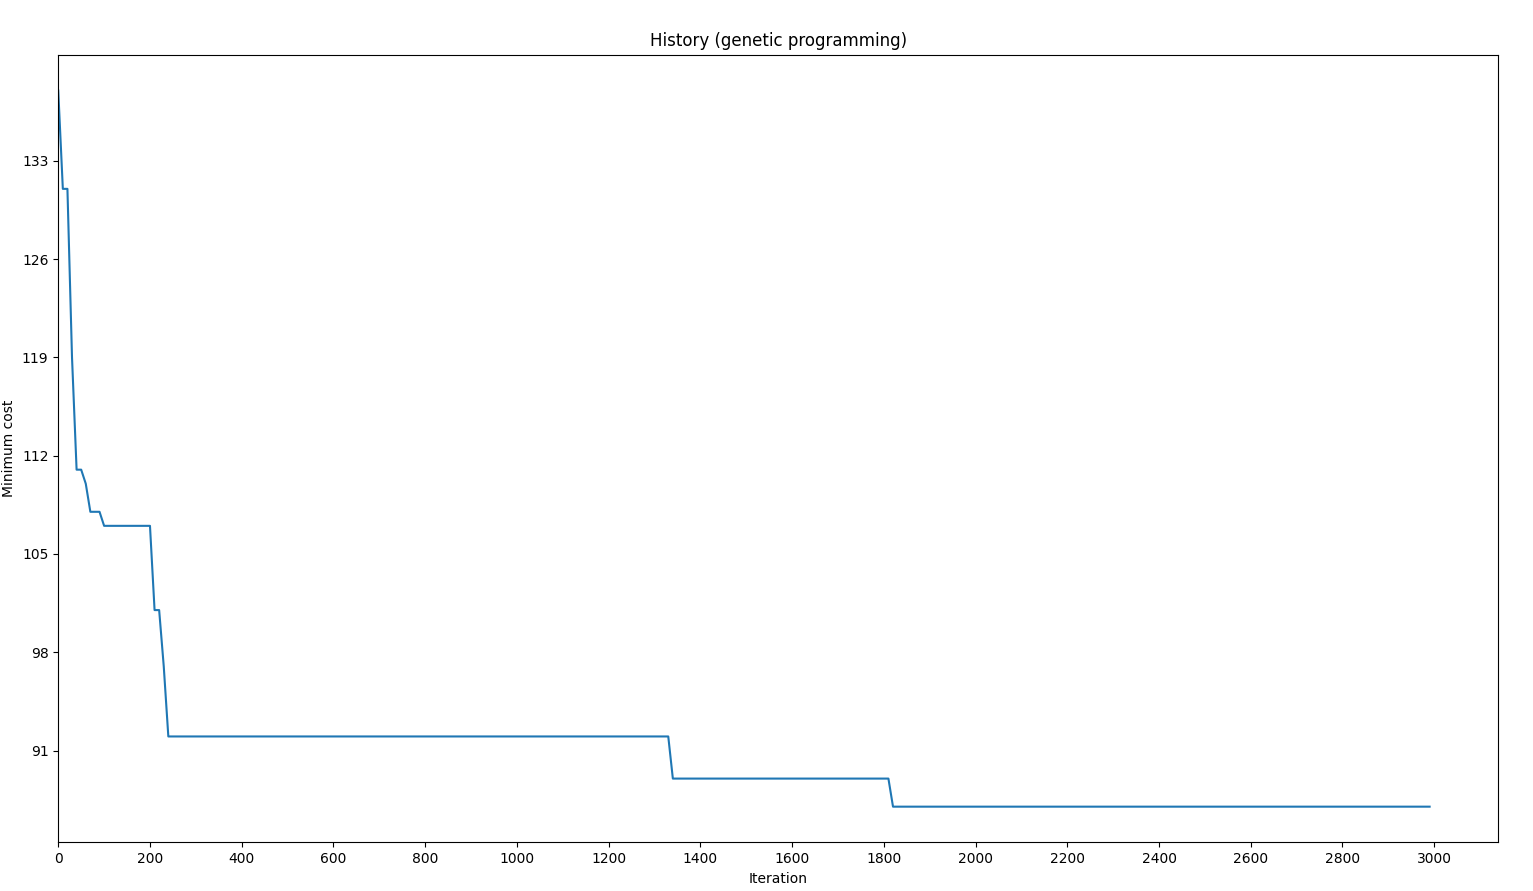
\includegraphics[scale=0.125]{Image/Snapshot/GeneticProgramming4}}}
\qquad
\subfloat[\centering iscrpna pretraga]{{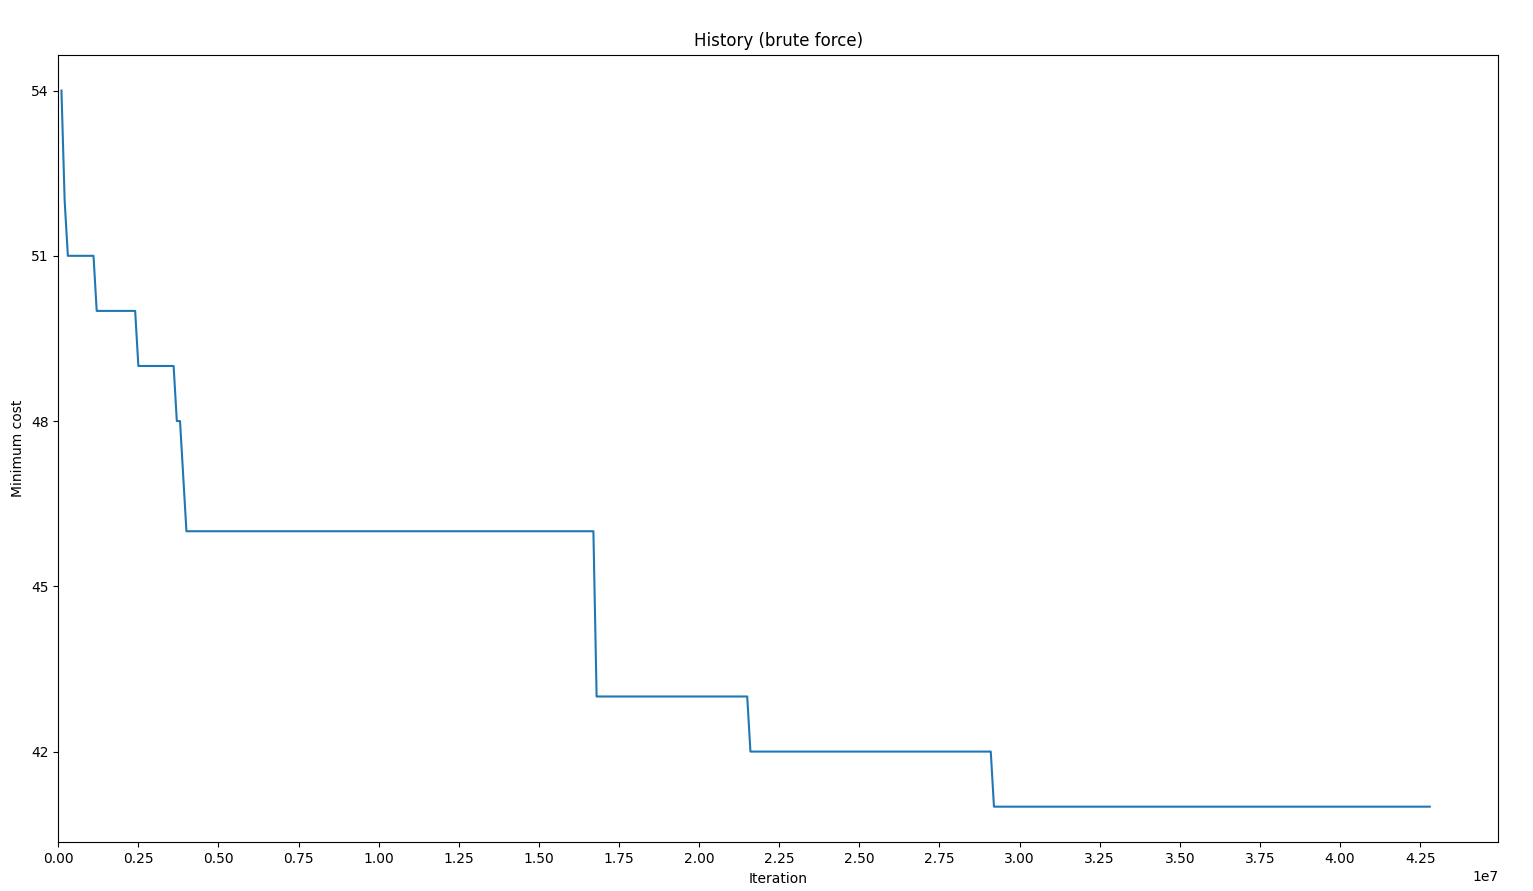
\includegraphics[scale=0.125]{Image/Snapshot/Bruteforce4}}}
\caption{Primena genetičkog programiranja i iscrpne pretrage}
\label{methodexample2}
\end{figure}

\section{Zaključak}

Korišćenje genetskog programiranja za nalaženje optimalnog načina alociranja registara možda ne daje rešenja brže od već razvijenih heurističkih algoritama \cite{OnLocalRegisterAllocation} \cite{RegisterAllocationByPuzzleSolving}. Razlog je nesigurnost u vremenu koji je potreban da se dostigne dobar rezultat. Ovo se može poboljšati drugim metodama selekcije, mutacije i ukrštanja, ali nesigurnost i dalje ostaje. Razvijena metoda ovde diskutovana daje dobra rešenja, ali sporo u poređenju sa drugim metodama.

\newpage

\bibliographystyle{plain}
\bibliography{DocumentationBibliography}

\end{document}
